\section{Terrain}

\begin{e1}
	
	\itemt{Comment le terrain affecte-t'il le \gls{cas}?}{
		
		Le terrain peut affecter les communications et la \gls{los}.
		
		Les unités \glspl{rw} sont particulièrement concernées. Le planificateur doit compenser ces limitations en implémentant des relais, ou intégrer ces limitations à la mission.
		
		La visibilité et le plafond peuvent affecter la décision d'employer des tactiques basse, moyenne ou haute altitude, ou l'utilisation de \glspl{rw}. Ces conditions affectent également la capacité du \gls{jtac} à voir la cible.
		
		Si des véhicules ennemis se déplacent, une colonne de fumée peut révéler leur emplacement.
		
		La visibilité a un impact plus important sur les armes à longue portée (bombe lisse, roquettes) que sur les armes à courte portée (canon, bombes freinées).
		
		Un brouillard épais a plus d'impact sur les attaques à bas niveau. Une visibilité réduite et une couche nuageuse importante peuvent restreindre l'emploi de l'armement \gls{eo}.
		
		L'acquisition de la cible est généralement plus facile lorsque le soleil se trouve derrière l'appareil qui attaque.
	}
	
	\begin{e2}
		
		\itemt{Masquage de la cible:}{
			
			Une cible masquée par le terrain, un immeuble ou une couverture naturelle peut être difficile à repérer. Une altitude plus élevée peut aider.
		}
		
		\itemt{Imagerie thermique:}{
			
			Un grand nombre de variables affecte l'efficacité de l'imagerie thermique. L'état de l'équipement, l'heure de la journée et l'arrière-plan doivent être pris en compte.
		}
		
		\itemt{Contraste et luminosité:}{
			
			Le contraste de la cible avec son arrière plan est un facteur critique lors de la recherche de cible. Une cible camouflée devant un arrière-plan de couleur similaire peut être impossible à détecter depuis une haute altitude ou une grande distance.
			
			Toutes les cibles, quelque soit le contraste, sont plus difficiles à repérer en condition de faible luminosité.
		}
		
		\itemt{Environnement montagneux:}{
			
			Un environnement montagneux peut forcer l'ennemi à concentrer ses forces sur les routes, dans les vallées, sur des pentes plus faibles ou dans de profond défilés, là ou le \gls{cas} est très efficace. 
			
			Cependant, ce type de terrain restreint également la direction d'attaque des appareils \gls{cas}. Le planificateur doit supposer que l'ennemi va concentrer ses défenses sur l'axe d'attaque le plus probable.
		}
		
		\itemt{Environnement désertique:}{
			
			Les appareils \gls{cas} sont rendus plus vulnérables par l'absence de couverture, et la dispersion des unités au sol.
		}
		
		\begin{e3}
			\itemt{Acquisition de la cible:}{
				En général, comme le contraste entre la cible et l'arrière plan est fort, la détection sera possible à plus longue portée.}
			\itemt{Emploi des armes:}{
				Un environnement désertique permettra généralement l'emploi des armes à leur portée maximale.}
			\itemt{Communications:}{
				En environnement désertique, les communications sont généralement possible à plus longue portée.}
			\itemt{Menaces:}{
				Les menaces seront également capables d'acquérir et d'engager les appareils \gls{cas} à portée maximale.}
			\itemt{Manque de références:}{
				Le désert, de par l'absence de références distinctes au sol, rend le talk-on et l'établissement d'\gls{ip} difficiles}
		\end{e3}
		
		\itemt{Jungle/forêt:}{
			Généralement, le contact avec l'ennemi se fera à très courte portée.
		}
		
		\begin{e3}
			\itemt{Acquisition de la cible:}{
			L'acquisition de la cible peut être rendue difficile, voire impossible, par la densité des arbres, pour l'appareil qui attaque comme pour le \gls{jtac}. Dans ces conditions, il appartient au \gls{gc} de marquer la cible. Un \gls{faca} en station peut également aider de par sa \gls{sa} supérieure.
		}
		\end{e3}
		
		\itemt{Environnement urbain:}{
			Le \gls{cas} en environnement présente des particularités uniques, parmi lesquelles la déconfliction en espace confiné, des \glspl{roe} particulières, la difficulté d'analyser la menace, la présence de non-combattants, le risque de dégâts collatéraux et l'augmentation du risque de tir fratricide.
		}
		
		\begin{e3}
			\itemt{Menaces:}{
				La ville offre d'excellent couvertures aux unités anti-aériennes.
				
				Les \glspl{sam} ou \gls{aaa} légers peuvent être employés depuis les toits.
				
				Le terrain encombré peut rendre l'acquisition des menaces difficile.
				
				Le placement des zones d'attente est rendu difficile par la dispersion des menaces dans une grande zone urbaine. Les \glspl{rw} nécessitent un secteur sécurisé de manière à pouvoir se déplacer est être moins prévisibles.
				
				Les \glspl{fw} établissent leur zone d'attente en terrain non-hostile, mais suffisamment proche de la ville que pour pouvoir assurer un support rapide.
			}
			
			\begin{e4}
				
				\itemt{Infrarouge et \glspl{nvg}:}{}
				\begin{e5}
					\item Les signatures infrarouges sont affectées par la proximité des bâtiments. La température généralement plus haute en environnement urbain affectent négativement le contraste infrarouge entre la cible et l'arrière-plan.
					\item Les lumières de la ville peuvent saturer les \glspl{nvg} et les rendre inutiles.
				\end{e5}
				
				\itemt{\gls{cc}:}{
					L'environnement urbain présente de gros problèmes de communications du fait des immeubles qui bloquent la \gls{los} et absorbent ou reflètent les signaux. L'utilisation d'un \gls{cc} aéroporté ou de relais permet d'en minimiser l'impact.
				}
				
				\itemt{Particularités propres au \gls{jtac}:}{
					Les hauts bâtiments rendent l'acquisition de la cible par le pilote difficile, et peuvent nécessiter l'emploi de \gls{fah} spécifiques. Des observateurs peuvent être placés sur les toits pour améliorer la vue d'ensemble.
				}
				
				\itemt{Efficacité:}{
					Un entraînement spécifique à l'environnement urbain est nécessaire pour que le \gls{jtac} y soit efficace.
					
					Historiquement, les engagements en zone urbaine se produisent dans 90\% des cas lorsque les troupes amies se trouvent à moins de 50 mètres des forces ennemies, et 80\% des blessures en zone urbaine proviennent des débris de verre dûs aux ondes de choc et aux surpression faisant suite à une explosion.
					
					Le \gls{jtac} doit porter une attention particulière à sélectionner l'armement approprié. La situation en zone urbaine change très rapidement, de bâtiment en bâtiment.
					
					Le \gls{jtac} peut utiliser les appareils de \gls{cas} ou le \gls{faca} pour engager des forces ennemies en dehors de la zone d'engagement, pour empêcher ces dernières de renforcer la ligne de front.
				}
				
				\itemt{Navigation:}{
					La navigation est plus difficile en ville. Les bâtiments ne sont pas indiqués sur les cartes. Les mouvements rapides peuvent embrouiller les observateurs au sol ou en l'air concernant les positions amies et ennemies.
				}
				
				\itemt{\gls{grg}/Grille urbaine:}{
					Des cartes ou des images détaillée de la zone urbaine peuvent être établies. Ces cartes ou ces images représentent la zone urbaine et peuvent contenir des bâtiments numérotés, les zones d'atterrissage pour les \glspl{rw}, des points de références, etc.
					
					C'est la responsabilité du \gls{gc} d'établir les cartes/images pour sa zone, et d'en assurer la gestion des versions ainsi que la diffusion. \textbf{Ces grilles doivent être établies en prenant en compte ce que les appareils de \gls{cas} pourront repérer le plus facilement (rivières, carrefours, bâtiments remarquables, ponts, etc.)}.
					
					Recommandations pour la création de \gls{grg}:
				}
				
				\begin{e5}
					\item L'image doit contenir une flèche pointant vers le nord, et être idéalement orientée avec le haut vers le nord.
					\item Les coordonnées est et nord doivent se trouver en haut et à gauche.
					\item Les bâtiments doivent être numérotés du nord-ouest au sud-est pour de grandes zones, ou dans le sens des aiguilles d'une montre à partir de l'objectif pour de plus petites zones.
				\end{e5}
				\efig{urbangrid}{Grille urbaine 1}
%				\efig[\textwidth][0.4\textheight]{grg1}{Grille urbaine 2 (merci à la \onethreetwo{})}
%				\efig[\textwidth][0.4\textheight]{grg3}{Grille urbaine 3 (merci à la \onethreetwo{})}
%				\efig[\textwidth][0.25\textheight]{grg4}{Grille urbaine 4 (merci à la \onethreetwo{})}
%				\efig[\textwidth][0.25\textheight]{grg5}{Grille urbaine 5 (merci à la \onethreetwo{})}
%				\efig[\textwidth][0.25\textheight]{grg6}{Grille urbaine 6 (merci à la \onethreetwo{})}
%				\efig{grg2}{Grille urbaine 7 (merci à la \onethreetwo{})}
				\begin{figure}[H]
					\centering 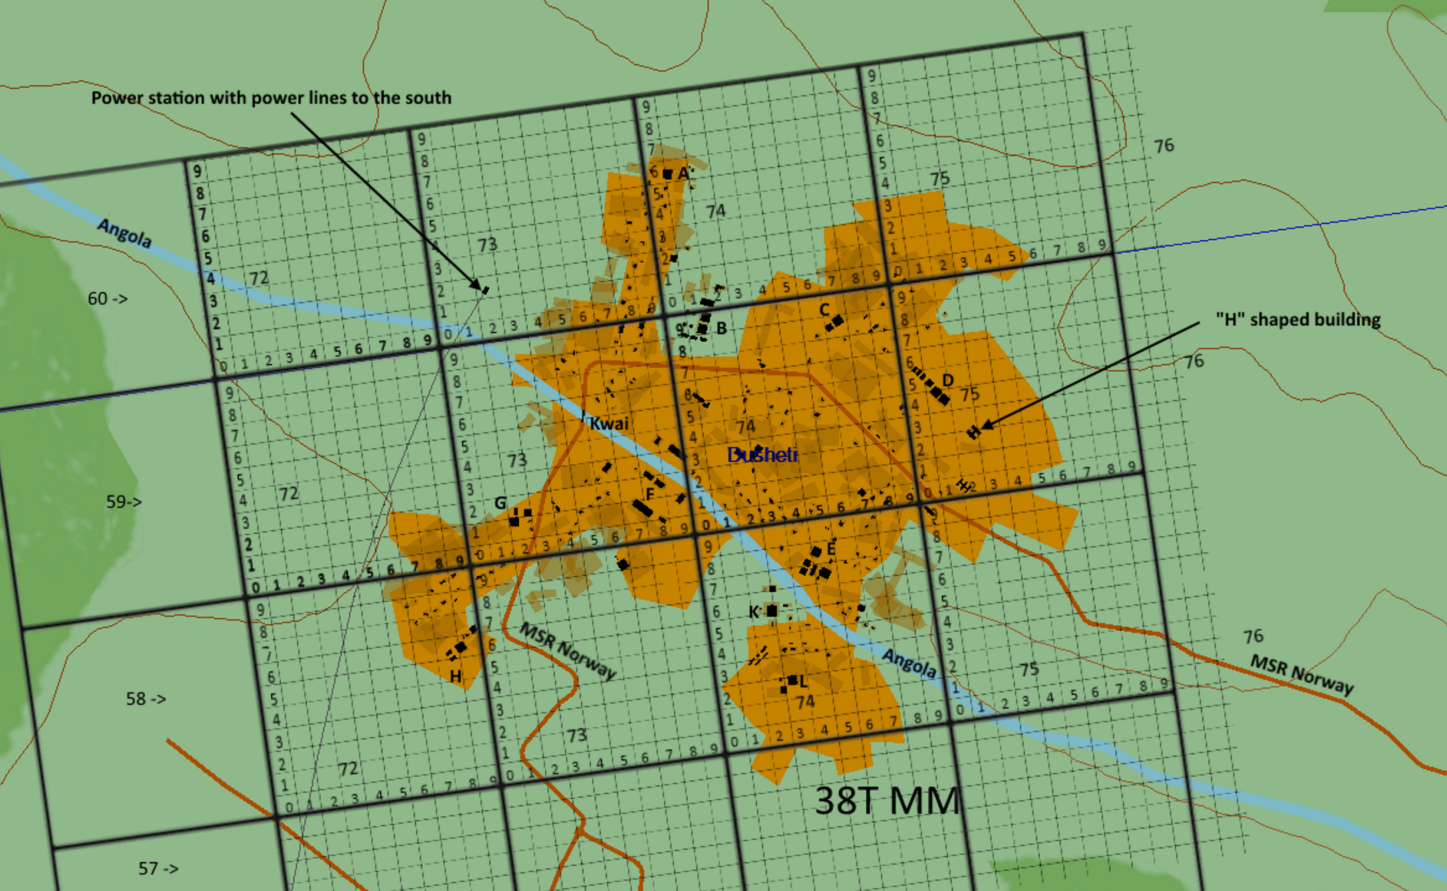
\includegraphics[width=\textwidth, max height=0.4\textheight, keepaspectratio]{grg1.png} \caption[Grille urbaine 2]{Grille urbaine 2 (merci à la \onethreetwo{}!)} \label{grg1}
				\end{figure}
				\begin{figure}[H]
					\centering 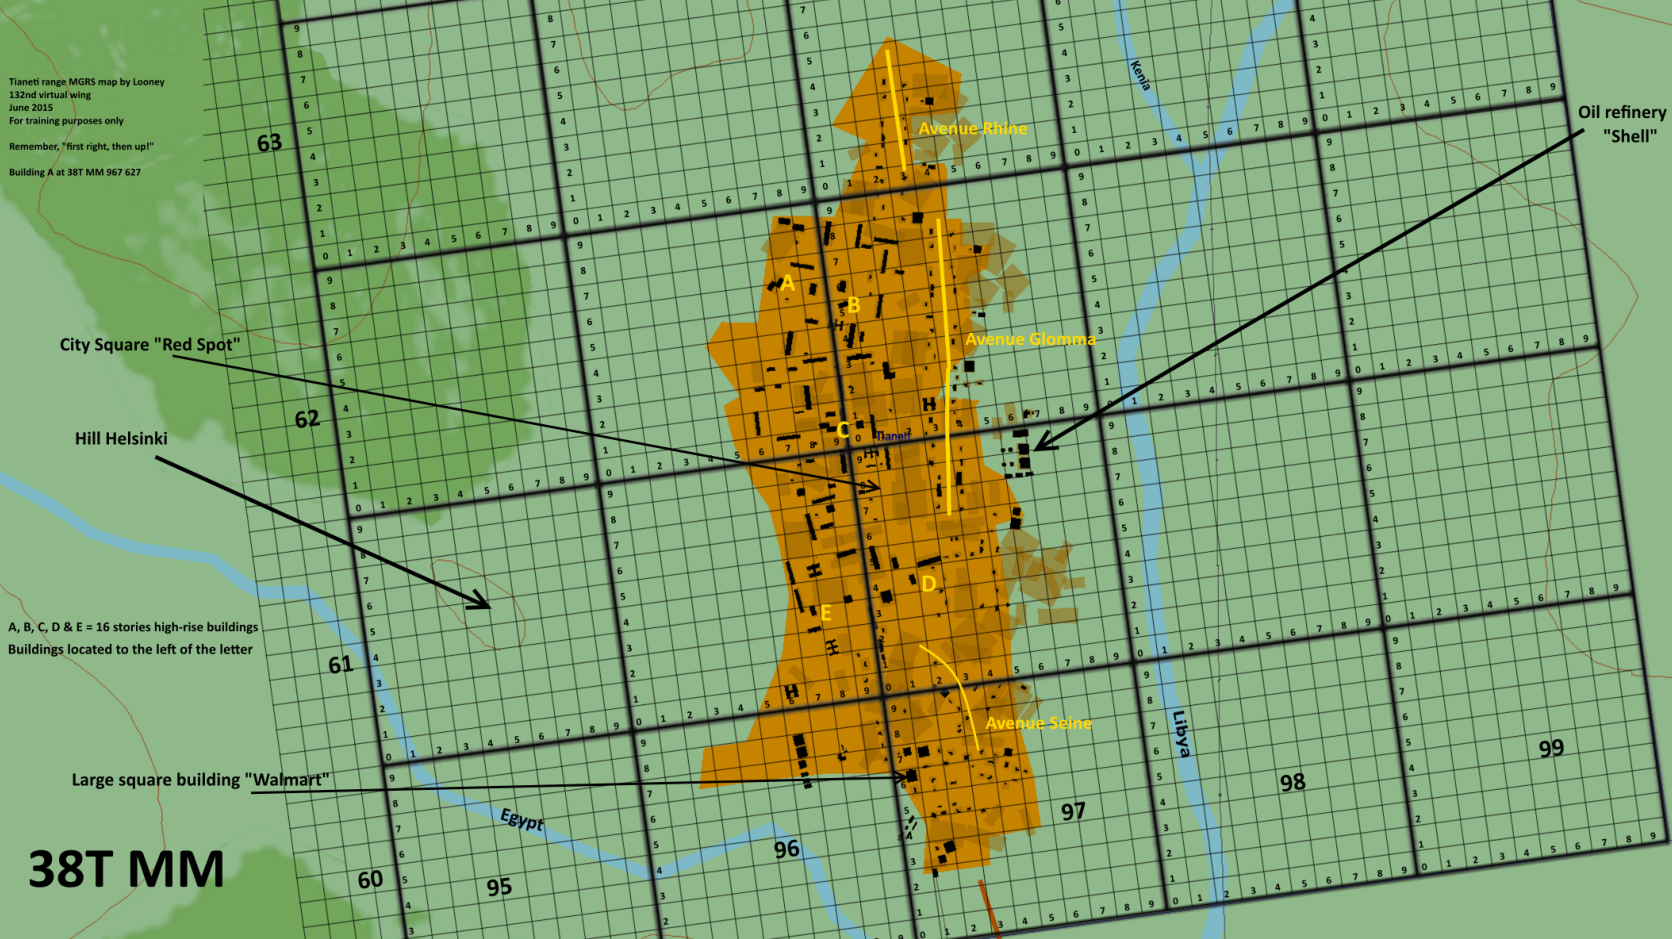
\includegraphics[width=\textwidth, max height=0.4\textheight, keepaspectratio]{grg3.png} \caption[Grille urbaine 3]{Grille urbaine 3 (merci à la \onethreetwo{}!)} \label{grg3}
				\end{figure}
				\begin{figure}[H]
					\centering 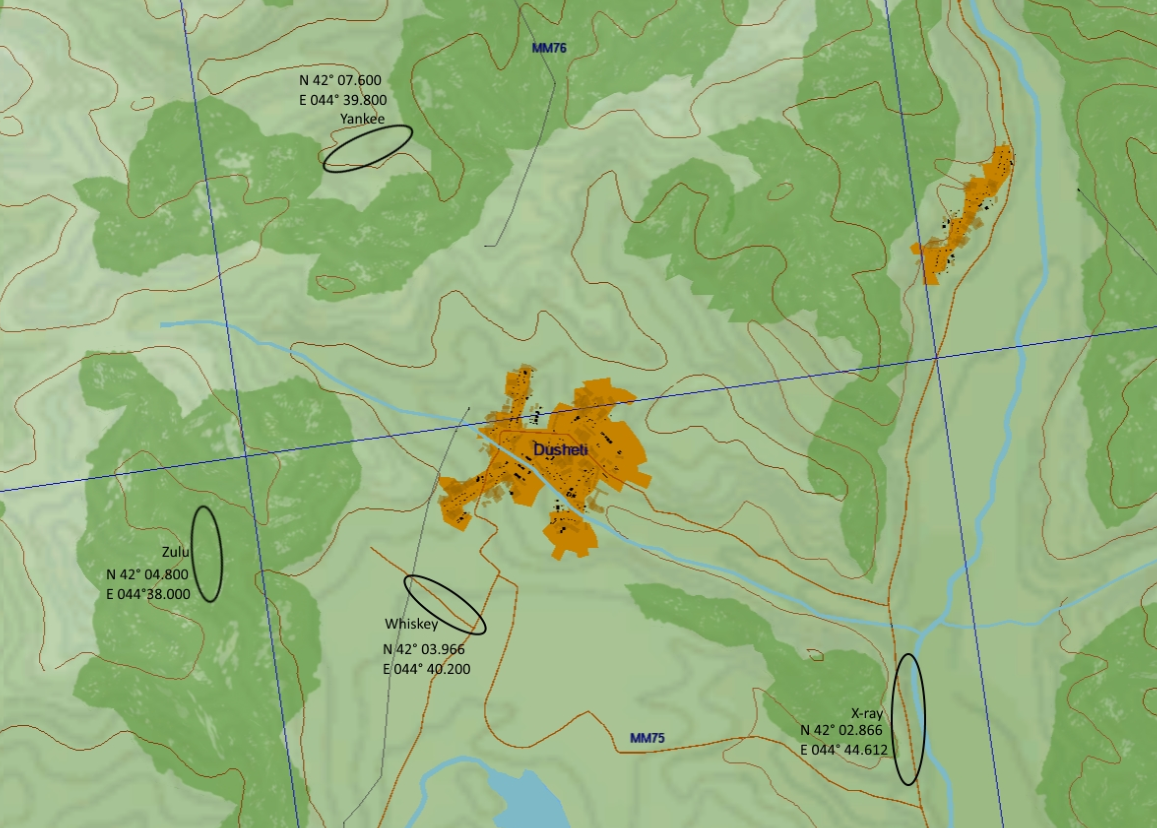
\includegraphics[width=\textwidth, max height=0.25\textheight, keepaspectratio]{grg4.png} \caption[Grille urbaine 4]{Grille urbaine 4 (merci à la \onethreetwo{}!)} \label{grg4}
				\end{figure}
				\begin{figure}[H]
					\centering 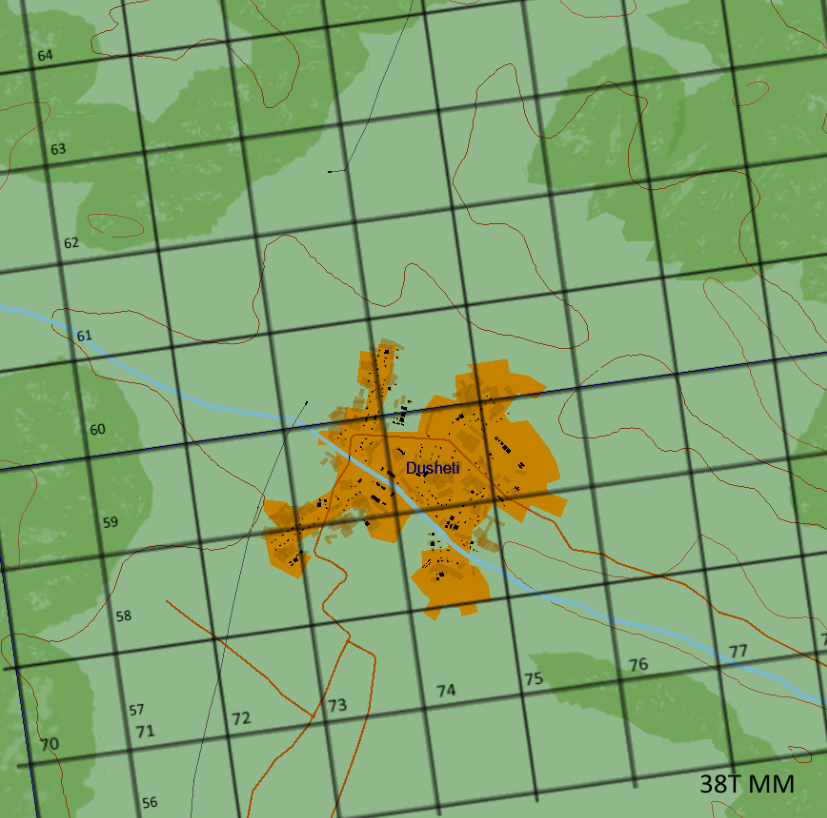
\includegraphics[width=\textwidth, max height=0.25\textheight, keepaspectratio]{grg5.png} \caption[Grille urbaine 5]{Grille urbaine 4 (merci à la \onethreetwo{}!)} \label{grg5}
				\end{figure}
				\begin{figure}[H]
					\centering 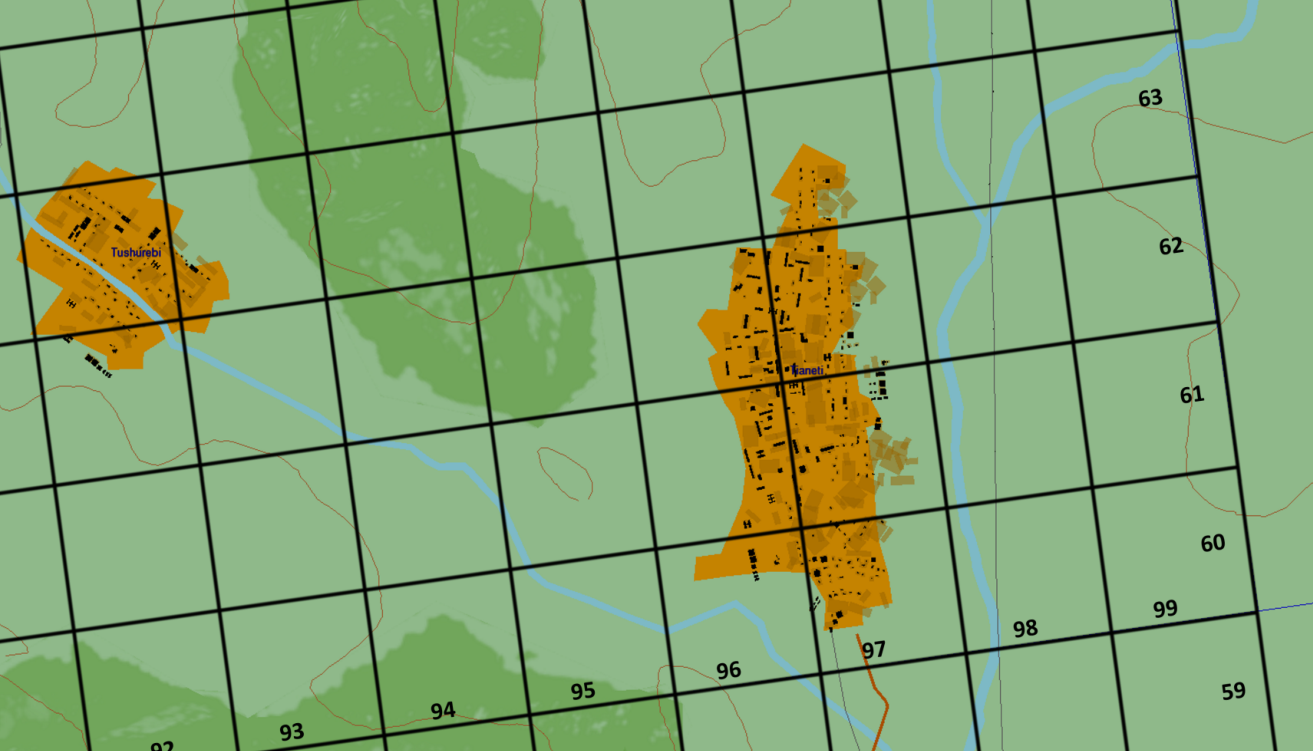
\includegraphics[width=\textwidth, max height=0.25\textheight, keepaspectratio]{grg6.png} \caption[Grille urbaine 6]{Grille urbaine 4 (merci à la \onethreetwo{}!)} \label{grg6}
				\end{figure}
				\begin{figure}[H]
					\centering 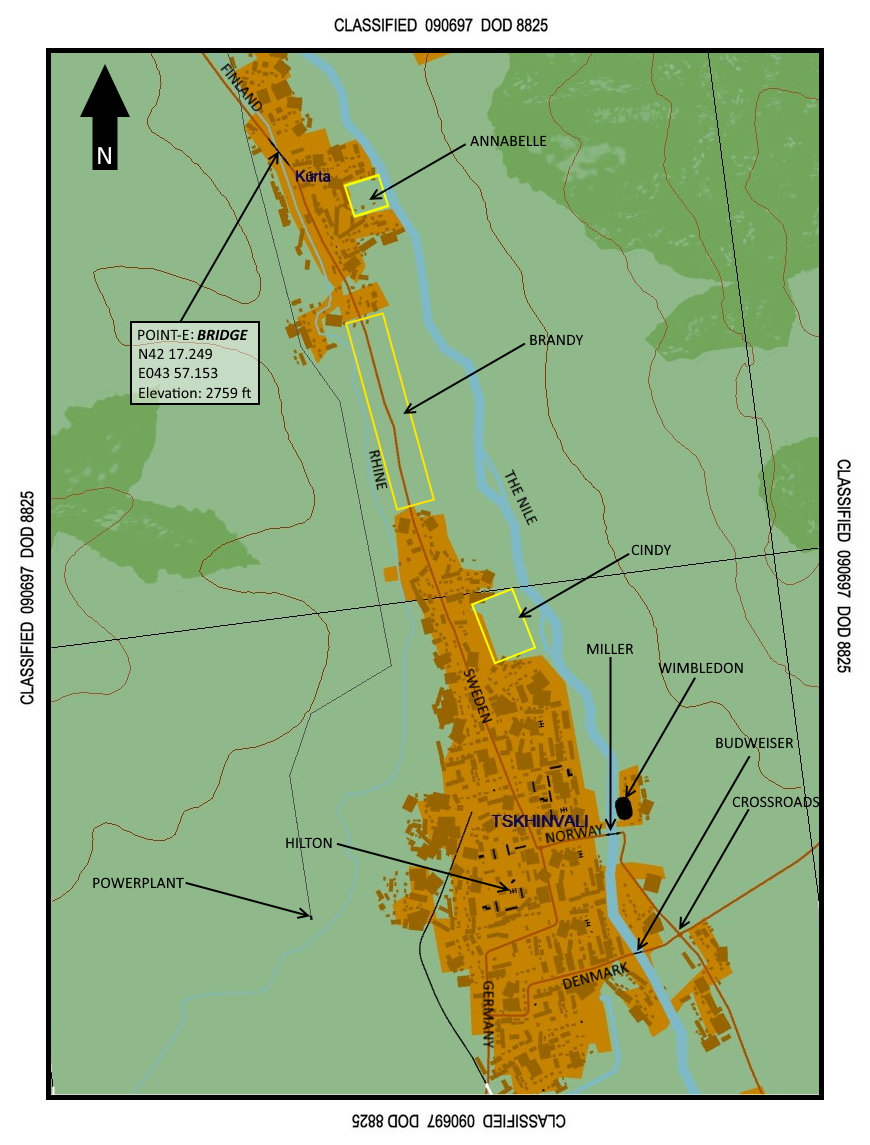
\includegraphics[width=\textwidth, max height=0.9\textheight, keepaspectratio]{grg2.png} \caption[Grille urbaine 7]{Grille urbaine 4 (merci à la \onethreetwo{}!)} \label{grg2}
				\end{figure}
				
				\newpage
				
				\itemt{\glspl{trp}:}{
					Des \glspl{trp} peuvent également être utilisés. Les \glspl{trp} sont générés en numérotant les bâtiments ou les particularités urbaines dans et autour de la zone de l'objectif. Ils peuvent être labellisés TRP\#1, TRP\#2, etc. Les \glspl{trp} permettent de passer ou interpréter un appel concernant un tir ennemi.
				}
				
				\efig{trp}{Target Reference Point}
				
				\itemt{Choix de l'armement:}{
					L'armement à utiliser en milieu urbain doit être choisi de manière à pouvoir tirer rapidement, de manière précise, et à minimiser les dommages collatéraux. Combiner les \glspl{rw} et les \glspl{rw} peut s'avérer être une tactique judicieuse: l'aptitude du \gls{fw} à acquérir et désigner une cible en zone urbaine peut être combiné avec la capacité du \gls{rw} à utilisé une \gls{pgm} de moindre puissance depuis une \gls{bp} sécurisée.
					
					Il faut adapter le type de munitions employées: un bombe à fragmentation, très efficace contre une concentration d'unité légèrement blindées en terrain ouvert, n'est pas un choix à considérer en zone urbaine.
				}
				
				\itemt{Exigences du \gls{sead}:}{
					Si la menace sol-air est importante, le \gls{cas} peut être réduit jusqu'à ce qu'elle soit suffisamment réduite. Le support \gls{sead} peut être nécessaire contre les défense sol-air ennemie, à l'intérieur comme à l'extérieur de la ville. Un \gls{sead} agressif et pro-actif peut être nécessaire au commencement d'une opération.
				}
				
			\end{e4}
			
			\itemt{Visibilité limitée, nuit et mauvaise météo:}{
				Une visibilité limitée ou une mauvaise météo alourdissent la charge de travail du pilote et demande un pilotage et une connaissance des procédures plus pointus. Les \ja{} et les pilotes doivent régulièrement s'entraîner ensembles dans ces mauvaises conditions pour espérer être efficaces.
				
				Il y a trois grandes catégories de visibilité restreinte:
			}
			
			\begin{e4}
				\itemt{Visuel:}{
					Pendant la nuit, les \ja{} et les pilotes doivent travailler avec beaucoup moins de lumières, et utiliser les feux ou les illuminations artificielles pour se coordonner. Si la menace le permet, les \gls{jtac} peuvent décider d'employer les lumières des appareils ou des flares.}
				\begin{e5}
					
					\item Planification pour le visuel:
					
					\begin{e6}
						
						\itemt{Météo et visibilité restreinte:}{
							Si le temps est clair et que la lune éclaire, l'utilisation de sources de lumière supplémentaire peut ne pas être nécessaire. Le fumée, le brouillard ou les précipitations dans la zone cible peuvent réduire la visibilité et obliger les appareils à manoeuvrer plus près des menaces.
						}
						
						\itemt{Plafond bas:}{
							Un plafond bas peut forcer les appareils à voler plus bas et rendre la déconfliction aux positions d'attente difficile.
						}
						
						\itemt{Terrain:}{
							Connaître le terrain est indispensable pour effectuer du \gls{cas} de nuit.
						}
						
						\itemt{Sans illuminations:}{
							Attaquer une cible sans illumination supplémentaire dépend de plusieurs choses:
						}
						\begin{e7}
							\item La nécessité d'attaquer une cible sur un point (personne, véhicule, ou endroit) ou une zone (ensemble de bâtiments, groupe de véhicules).
							\item Lumière ambiante sur la zone cible.
							\item Cible illuminée ou pas.
							\item Distance oblique minimale due à la menace.
							\item Restrictions propres au théâtre d'opération.
						\end{e7}
						
						\itemt{Conditions changeantes (Aube/Crépuscule):}{
							A l'aube et au crépuscule, les \ja{} et les pilotes doivent d'adapter à des conditions qui changent rapidement. Il peut être nécessaire de changer la géométrie de l'attaque pour s'adapter aux nouvelles conditions.
						}
						
						\itemt{Illumination artificielle:}{
							Dans la plupart des cas, les \ja{} et les pilotes utiliseront des \glspl{nvg} ou un \gls{flir}. Les flares sont indispensables pour des opérations de nuit sans \glspl{nvg} ou \gls{flir}. \textbf{Si possible, il ne faut pas éclairer les positions amies de nuit}.
						}
						
						\important{Toute illumination artificielle de la zone de combat de nuit doit préalablement être approuvée par le \gls{jtac}.}
						
						\begin{e7}
							\itemt{Fusée éclairante tirée depuis le sol:}{
								Ces fusées n'éclairent pas aussi fort ni aussi longtemps qu'une LUU-2 (ou équivalent).
							}
							\itemt{LUU-2 (ou équivalent):}{
							Ces fusées sont prévues pour illuminer une zone pendant environ 5 minutes.
							}
							\itemt{Roquette éclairante:}{
							Une roquette éclairante est prévue pour illuminer la zone pendant environ 2 minutes.
							}
						\end{e7}
						
						\itemt{Marques:}{
							Les fusées au phosphore sont régulièrement utilisées comme marque. La lumière ambiante peut se refléter dessus et les rendre visible, même de nuit.
						}
						
					\end{e6}
					
					\itemt{Exécution du visuel:}{
						La positions des alliés, le vent et la menace détermineront la géométrie d'attaque et l'armement employé.
					}
					
				\end{e5}
				
				\itemt{Assistance système:}{
					De nuit, l'acquisition de la cible aidée par le système embarqué est utilisé est généralement préférée.
				}
				
				\begin{e5}
					\itemt{Laser:}{
						Les procédures de nuit pour la désignation laser sont identiques aux procédures de jour.
					}
					\itemt{\gls{eo}/\gls{ir}:}{
						La couverture nuageuse, les précipitations et les conditions du champ de bataille (fumée, poussière, ou autre) peuvent dégrader les performances infrarouge ou électro-optiques.
					}
					\itemt{\gls{hmcs}:}{
						Dans un rôle air-sol, le \gls{hmcs} est utilisé conjointement aux autres senseurs pour augmenter la réactivité et la \gls{sa} du pilote.
					}
				\end{e5}
				
				\itemt{Emploi des \glspl{nvg}:}{
					Les \glspl{nvg} sont un senseur supplémentaire pour le pilote. Les \ja{} doivent être équipés de pointeurs \gls{ir} pour en exploiter le plein potentiel.
				}
				
				\begin{e5}
					
					\item Préparation d'une mission avec \glspl{nvg}:
					
					\begin{e6}
						
						\itemt{Météo:}{
							Un ciel couvert peut diminuer la luminosité ambiante et marquer la silhouette de l'appareil pour les forces au sol.
						}
						
						\itemt{Marques:}{
							Un pointeur \gls{ir} est le complément parfait des \gls{nvg}. Cependant, une coordination supplémentaire est nécessaire pendant la corrélation pour s'assurer que le pilote a bien acquis le bon bout du pointeur.
						}
						
						\itemt{Roquette, artillerie:}{
							La chaleur produite par l'explosion initiale de la roquette ou de l'obus au phosphore sera clairement visible aux \glspl{nvg}.
						}
						
					\end{e6}
					
					\item Exécution d'une mission avec \glspl{nvg}:
					
					\begin{e6}
						
						\itemt{Armement embarqué:}{
							En général, toute les bombes lisses créeront à l'impact un flash de lumière qui peut être utilisé comme marque. L'explosion réchauffera le sol alentour pour un temps, ce qui peut également être utilisé comme marque \gls{ir}.
						}
						
						\itemt{Équipement \gls{ir} des troupes au sol:}{
							En fonction des conditions, tout le faisceau sera visible, ou juste la partie autour de la cible. Le faisceau sera étroit à sa source, sur le \gls{jtac}, et diffus sur la cible. 
							
							L'illumination de la cible par le \gls{jtac} doit être la plus courte possible, de manière à ne pas compromettre la position de ce dernier si l'ennemi est également équipé de \glspl{nvg}.
						}
					
						\begin{minipage}{\linewidth}
							
							\itemt{Équipement \gls{ir} aéroporté:}{
								Ces équipements fonctionnes généralement très bien depuis une altitude moyenne.
								
								Une lumière ambiante élevée réduira leurs performances mais ne les empêchera pas de fonctionner.
								
								Ces équipements peuvent être utilisés pour augmenter la \gls{sa} du \ja{} en marquant la cible, ou en pointant sur la même cible pour corrélation.}
							
							\vskip5mm
							
							\important{Les appareils équipés de pointeurs \gls{ir} doivent se coordonner avec le \gls{jtac} avant de pouvoir les utiliser}
							
						\end{minipage}
						
					\end{e6}
					
				\end{e5}
				
				\itemt{Marquage des unités amies:}{
					
				Les forces au sol alliées peuvent marquer leur position par différents moyens.}
			
				\begin{e5}
					\item Pointeur \gls{ir}:\\
					\itemt{Marqueur \gls{ir}:}{
						Pas d'application dans DCS.
					}
					
					\itemt{GLINT tape:}{
						Pas d'application dans DCS.
					}
					
				\end{e5}
				
			\end{e4}
			
			\itemt{Paramètres d'autorisations \gls{bot} avec marqueur \gls{ir} au sol:}{
				Lors de l'emploi de marqueurs \gls{ir} au sol, les pilotes devront appeler "VISUEL" lors de l'acquisition de la position amie ou "TALLY" pour l'acquisition de la position ennemie, et "CONTACT SPARKLE" à chaque passe avant d'obtenir l'autorisation de tir. La brevity propre à l'utilisation de l'\gls{ir} doit être maintenue jusqu'à l'appel "CEASE SPARKLE".
			}
			
			\itemt{CAS brief:}{
				Si le \gls{jtac} à l'intention d'utiliser un pointeur \gls{ir}, ce sera indiqué dans le CAS brief, ligne 7, "Type de marque", comme "IR" ou "Pointeur IR".
			}
			
		\end{e3}
	\end{e2}
\end{e1}